\documentclass{article}

% Packages
% ---
\usepackage{amsmath,amssymb,amsthm} 	% Advanced math typesetting
% \usepackage[utf8]{inputenc} 	% Unicode support (Umlauts etc.)
\usepackage[USenglish]{babel} 	% Change hyphenation rules
\usepackage{hyperref} 				% Add a link to your document
\usepackage{graphicx}				% Add pictures to your document
\graphicspath{ {./images/} }		% image directory

% Typewriter settings for code
\usepackage{listings} 				% Source code formatting and highlighting
\lstset{basicstyle=\ttfamily}		%Typewriter font for code writing


\usepackage{enumitem}

% Margins
\usepackage{geometry}
\geometry{margin=1in}


\usepackage{float}
\restylefloat{figure}
\usepackage{mathabx}
\usepackage{fancyhdr}
\usepackage[dvipsnames]{xcolor}
\usepackage{scrextend}

% Siderules for digressions/examples
\usepackage{mdframed}
\newmdenv[
topline=false,
bottomline=false,
skipabove=\topsep,
skipbelow=\topsep
]{siderules}

% Colors
\definecolor{blu}{rgb}{0,0,1}
\def\blu#1{{\color{blu}#1}}
\definecolor{gre}{rgb}{0,.5,0}
\def\gre#1{{\color{gre}#1}}
\definecolor{red}{rgb}{1,0,0}
\def\red#1{{\color{red}#1}}
\def\norm#1{\|#1\|}


% Headers
\pagestyle{fancy}
\fancyhf{}
\lhead{\bf CPSC 322 \\ Week 11 }
\rhead{\bf Jeremi Do Dinh \\ 61985628}
\rfoot{Page \thepage}

% Graph drawing tools
\usepackage{tikz}						
\usetikzlibrary {positioning}

\usepackage{breqn}
\usepackage{multicol} 				% Multiple column functionality
\usepackage{blindtext}

% Figure shortcut
\newcommand{\centerfig}[2]{\begin{center}\includegraphics[width=#1\textwidth]{#2}\end{center}}

\begin{document}

\section*{Lecture 28 - BNet Inference}
\url{https://www.cs.ubc.ca/~jordon/teaching/cpsc322/2019w2/lectures/lecture28.pdf}
\subsubsection*{Goals}
\begin{itemize}
	\item Define factors. Derive new factors from existing factors. Apply operations to factors, including assigning, summing out and multiplying factors.
	\item Carry out variable elimination by using factor representation and using the factor operations. Use techniques to simplify variable elimination.
\end{itemize}

\subsection*{BNet Inference}
Our goal in BNet inference is to compute the probabilities of the variables in a belief network:
\begin{itemize}
	\item What is the posterior distribution over one or more variables, conditioned on one or more observed variables?
\end{itemize}
\subsubsection*{BNets in General}
Suppose we have that the variables in the belief network are $ \{X_1, \dots, X_n\} $. We also have a variable $ Z $ which we call the "query" variable. \\
\\
We have variables $ Y_1 = v_1, \dots, Y_j = v_j $ which are the \textbf{observed v\blu{arg1}ariables}, and their corresponding observed values. $ Z_1, \dots, Z_k $ are the remaining variables. \\
\\
We wish to compute:
\begin{align*}
P(Z | Y_1 = v_1, \dots, Y_j = v_j)
\end{align*}
\begin{siderules}
We bring back the example of the fire alarm, where we had the following belief network:
\centerfig{0.3}{BNet-2}
In this case we may wish to compute: $ P(L | S = t , R = f)$. From marginalization we know that:
\begin{align*}
 \blu{P(L | S = t , R = f)} &= \frac{\color{Fuchsia}P(L , S = t , R = f)}{\gre{P(S = t , R = f)}}
\end{align*}
An we are given the necessary data to do so:
\centerfig{0.7}{BNet-3}
\end{siderules}
\textbf{In general, we have}
\begin{align*}
P(Z | Y_1 = v_1, \dots, Y_j = v_j) &= \frac{P(Z, Y_1 = v_1, \dots, Y_j = v_j)}{P(Y_1 = v_1, \dots, Y_j = v_j)} \\
&= \frac{P(Z, Y_1 = v_1, \dots, Y_j = v_j)}{\sum_{Z}P(Z,Y_1 = v_1, \dots, Y_j = v_j)}
\end{align*}
However we only need to \textbf{compute the \blu{numerator}}, and then \textbf{normalize}. This can be framed in terms of \textbf{operations between \blu{factors}} (that satisfy the semantics of probability)

\subsection*{Factors}
\textbf{Def:} A \textbf{\textit{Factor}} is a representation of a function from a tuple of random variables into a number:
\begin{itemize}
	\item We will denote the factor $ f $ of random variables $ X_1, \dots, X_j $ as $ f(X_1, \dots, X_j) $
\end{itemize}
A Factors can denote:
\begin{itemize}[label = $ \rightarrow $]
	\item One distribution
	\item One partial distribution
	\item Several distributions
	\item Several partial distributions
\end{itemize}
over the given tuple of variables.
\begin{siderules}
	\textbf{Examples}
	\begin{itemize}
		\item Distribution\\
		$ P(X_1, X_2) $ is a factor $ f(X_1, X_2) $
	\begin{center}
		\begin{tabular}{|c|c|c|}
			\hline
			$ X_1 $ & $ X_2 $ & $  f(X_1, X_2) $\\
			\hline
			T & T & $ 0.12 $ \\
			\hline
			T & F & $ 0.08 $ \\
			\hline
			F & T & $ 0.08 $ \\
			\hline
			F & F & $ 0.72 $ \\
			\hline
		\end{tabular}
	\end{center}

	\item Partial distribution\\
	$ P(X_1, X_2 = F) $ is a factor $ f(X_1)_{X_2 = F} $
	\begin{center}
		\begin{tabular}{|c|c|c|}
			\hline
			$ X_1 $ & $ X_2 $ & $  f(X_1)_{X_2 = F}$\\
			\hline
			F & T & $ 0.08 $ \\
			\hline
			F & F & $ 0.72 $ \\
			\hline
		\end{tabular}
	\end{center}
\item Set of Distributions\\
$ P(X | Z,Y) $ is a factor $ f(X,Z,Y) $
\item Set of partial Distributions\\
$ P(X_1, X_3 = v_3 | X_2) $ is a factor $ f(X_1, X_2)_{X_3 = v_3}  $
	\end{itemize}
	
	\end{siderules}
\subsection*{Operations on factors}
We can make new factors based on existing factors. 
\subsubsection*{Variable assignment}
To begin with, for instance it is possible to assign some, if not all of the variables to a factor. This assignment then reduces the factor dimension (i.e.: the number of variables in a factor). \\
\\
For instance if we have a factor $ f(X,Y,Z) $, what would be the result of assigning $ X = t $? TFAE:
\begin{align*}
f(X=t, Y, Z) = f(X,Y,Z)_{X=t} = f(Y,Z)
\end{align*}
\centerfig{0.3}{BNet-4}
\subsubsection*{Summing out a variable example}
We can \textbf{\textit{sum out a variable}}. WLOG let that variable be $ X_1 $, with domain $ \{v_1, \dots, v_k\} $. We can sum it out from factor $ f(X_1, \dots, X_j) $ resulting in a factor on $ X_2, \dots, X_j $ defined by:
\begin{align*}
\left( \sum_{X_1} f \right)\left( X_2, \dots, X_j \right) &= f(X_1 = v_1,X_2, \dots, X_j) + \dots + f(X_1 = v_k,X_2, \dots, X_j)
\end{align*}
\centerfig{0.8}{BNet-5}
\subsubsection*{Multiplying factors}
Factors can also be multiplied together. The \textbf{\textit{product}} of a factor $ f_1(A,B) $ and $ f_2(B,C) $ where $ B $ is the variable in common is the factor $ f_1 \times f_2(A,B,C) $ defined by:
\begin{align*}
 f_1(A,B) f_2(B,C) &= (f_1 \times f_2)(A,B,C)
\end{align*}
Notes:
\begin{itemize}
	\item It is defined on all $ A,B,C $ triples, obtained by multiplying together the appropriate pair of entries from $ f_1 $ and $ f_2 $.
	\item $ A,B,C $ can be sets of variables.
\end{itemize}

\subsection*{Intro to Variable Elimination}
Suppose we again have the scenario from above:\\
\\
The variables in the belief network are $ \{X_1, \dots, X_n\} $. $ Z $ is the query variable. \\
\\
We have variables $ Y_1 = v_1, \dots, Y_j = v_j $ which are the \textbf{observed variables}, and their corresponding observed values. $ Z_1, \dots, Z_k $ are the remaining variables. \\
\\
We want to compute:
\begin{align*}
P(Z | Y_1 = v_1, \dots, Y_j = v_j)\\
\intertext{We have then showed that what really need to be computed is:}
P(Z, Y_1 = v_1, \dots, Y_j = v_j)
\end{align*}
And this expression can be computed in terms of operations between the factors (that satisfy the semantics of probability).\\
\\
If we express the joint distribution as a single factor:
\begin{align*}
f(Z, \gre{Y_1, \dots , Y_j}, {\color{Fuchsia}Z_1, \dots, Z_k})
\end{align*}
Then we can compute $ P(Z, Y_1 = v_1, \dots, Y_j = v_j) $ by:\begin{itemize}
	\item \gre{\textbf{Assigning} $ Y_1 = v_1, \dots, Y_j =v_j$}
	\item {\color{Fuchsia}\textbf{Summing out} the variables $ Z_1, \dots, Z_k$}
\end{itemize}
\begin{align*}
P(Z, Y_1 = v_1, \dots, Y_j = v_j) &= \sum_{Z_k} \dots \sum_{Z_1} f(Z, Y_1, \dots , Y_j, Z_1, \dots, Z_k)_{Y_1 = v_1, \dots, Y_j = v_j}
\end{align*}
However, the joint distribution is too big to sum this for large problems. Thus we need to employ other strategies. 
\newpage
\section*{Lecture 29 - Variable Elimination}
\url{https://www.cs.ubc.ca/~jordon/teaching/cpsc322/2019w2/lectures/lecture29.pdf}
From the previous section we derived that:
\begin{align*}
P(Z, Y_1 = v_1, \dots, Y_j = v_j) &= \sum_{Z_k} \dots \sum_{Z_1} f(Z, Y_1, \dots , Y_j, Z_1, \dots, Z_k)_{Y_1 = v_1, \dots, Y_j = v_j}
\end{align*}
But the whole point of BNets was to get rid of the JPD. Using the chain rule and the definition of a BNet we can write $ P(X_1, \dots, X_n) $ as:
\begin{align*}
\prod_{i=1}^n P(X_1|\underbrace{\text{par}(X_1)}_{\text{parents of }X_i})
\end{align*}
 Using the chain rule we can also express the joint factor as a product of factors:
 \begin{align*}
 f(Z, \gre{Y_1, \dots , Y_j}, \blu{Z_1, \dots, Z_k}) &= \prod_{i=1}^n f(X_i | \text{par}(X_i)) \\
 P(Z, Y_1 = v_1, \dots, Y_j = v_j) &= \sum_{Z_k} \dots \sum_{Z_1} \prod_{i=1}^n f(X_i | \text{par}(X_i)) _{Y_1 = v_1, \dots, Y_j = v_j}
 \end{align*}
We therefore observe that inference in belief networks reduces to computing the \textbf{sum of products}. The algorithm consequently is:
\begin{enumerate}
	\item Construct a factor for each conditional probability
	\item In each factor \blu{assign} the observed variables to their observed values. 
	\item Multiply the factors. 
	\item for each of the other variables $ Z_i \in \{Z_1, \dots, Z_k\} $, \textbf{\blu{sum out}} $ Z_i $
\end{enumerate}
\subsubsection*{How to simplify the Computation?}
Let's assumes we have turned the CPTs into factors, and performed the assignments. We can focus on a basic case, to illustrate the decomposition. This case takes form when $ k =1$, and the distribution function is:
\begin{align*}
\sum_{Z_1} \prod_{i=1}^{n} f(\text{vars}(X_i))
\end{align*}
We have that in order to compute this efficiently, we first need to factor out the terms that do not involve $ Z_1 $. The above statement then becomes:
\begin{align*}
\left(  \prod_{i: Z_1 \notin \text{vars}(X_i)} f(\text{vars}(X_i))   \right) \cdot \left( \sum_{Z_1} \prod_{i: Z_1 \in \text{vars}(X_i)} f(\text{vars}(X_i)) \right)
\end{align*}
This is illustrated by the following specific case:
\begin{align*}
\sum_A f(C,D) \times f(A,B,D) \times f(E,A) \times f(D) &= \\
  f(C,D) \times f(D) \times \sum_A f(A,B,D) \times f(E,A) 
\end{align*}
This simplification is similar to what you can do in basic algebra with multiplication and addition:
\begin{itemize}
	\item It takes 14 multiplications or additions to evaluate the expression:
	\begin{align*}
	a b + a c + a d + a e h + a f h + ag h
	\end{align*}
	\item This expression be evaluated more efficiently (only 7 operations)
	\begin{align*}
	a \times (b + c + d + h \times (e + f + g))
	\end{align*}
\end{itemize}
There also is numerous ways in which it is possible to simplify the expression. 
\subsubsection*{Variable elimination algorithm}
Given 
\begin{align*}
f(Z, \gre{Y_1, \dots , Y_j}, {\color{Fuchsia}Z_1, \dots, Z_k})
\end{align*}
To compute:
\begin{align*}
P(Z | Y_1 = v_1, \dots, Y_j = v_j)
\end{align*}
\begin{enumerate}
	\item \blu{Construct a factor} for each conditional probability.
	\item Set the \blu{observed variables} to their observed values
	\item Given an \blu{elimination ordering, simplify/decompose} sum of products
	\item \blu{Perform products} and \blu{sum out} $ Z_i $
	\item \blu{Multiply} the remaining factors (All the remaining factors are in $ Z $ as we would've assigned all the evidence variables, and summed out all of the others).
	\item \blu{Normalize}: divide the resulting factor $ f(Z) $ by $ \sum_Z f(Z) $
\end{enumerate}

\begin{siderules}
	\textbf{Example}\\
	\\
	Consider the following BNet:
	\centerfig{0.15}{BNet-6}
	Suppose we want to compute $ P(G | H = h_1) $. We know that:
	\begin{align*}
	P(G, H) &= \sum_{A, B,C,D,E,F,I} P(A,B,C,D,E,F,G,H,I) \\
	\intertext{Using the chain rule, and conditional probability, we obrain the following decomposition:}
	 &= \sum_{A, B,C,D,E,F,I} P(A)P(B|A)P(C)P(D|B,C)P(E | C)P(F | D) P(G|E, F) P(H|G) P(I|G) \\
	 \intertext{We use factors now to represent the probabilities:}	 \
	 &=  \sum_{A, B,C,D,E,F,I}f_0(A)f_1(A,B)f_2(C)f_3(D, B, C)f_4(E,C) f_5(F,D) f_6(G,F,E) f_7(H,G)f_8(I,G) \\
	 \intertext{We have ovserved $ H = h_1 $, thus the expression simplifies to:}
	 &=  \sum_{A, B,C,D,E,F,I}f_0(A)f_1(A,B)f_2(C)f_3(D, B, C)f_4(E,C) f_5(F,D) f_6(G,F,E) {\color{Magenta}f_9(G)}f_8(I,G) \\
	 \intertext{We employ an elimination ordering of $ A, C, E, I, B, D, F  $:}
	 &=f_9(G)\sum_F \sum_D f_5(F,D) \sum_B  \sum_I f_8(I,G) \sum_E f_6(G,F,E) \sum_C f_2(C) f_3(D, B, C)f_4(E,C)  \cdot  \\ & \quad \quad \quad \cdot \underbrace{\sum_A f_0(A)f_1(A,B)}_{{\color{Magenta}=f_{10}(B)}}\\
	 &= f_9(G)\sum_F \sum_D f_5(F,D) \sum_B  {\color{Magenta}f_{10}(B)} \sum_I f_8(I,G) \sum_E f_6(G,F,E) \underbrace{\sum_C f_2(C) f_3(D, B, C)f_4(E,C)}_{{\color{Magenta}=f_{12}(B,D,E)}} \\
	 &= f_9(G)\sum_F \sum_D f_5(F,D) \sum_B  f_{10}(B) \sum_I f_8(I,G) \underbrace{\sum_E f_6(G,F,E) {\color{Magenta}f_{12}(B,D,E)}}_{\color{Magenta}= f_{13}(B,D,F,G)}\\
	 &=f_9(G)\sum_F \sum_D f_5(F,D) \sum_B  f_{10}(B) {\color{Magenta}f_{13}(B,D,F,G)} \underbrace{\sum_I f_8(I,G)}_{\color{Magenta}=f_{14}(G)} \\
	 &=f_9(G){\color{Magenta}f_{14}(G)}\sum_F \sum_D f_5(F,D) \underbrace{\sum_B  f_{10}(B) f_{13}(B,D,F,G)}_{\color{Magenta}=f_{15}(D,F,G)}\\
	 &= f_9(G)f_{14}(G)\sum_F\underbrace{ \sum_D f_5(F,D) {\color{Magenta}f_{15}(D,F,G)}}_{\color{Magenta}=f_{16}(F,G)} \\
	 &=f_9(G)f_{14}(G)\underbrace{\sum_F{\color{Magenta}f_{16}(F,G)}}_{\color{Magenta}=f_{17}(G)}\\
	 &= f_9(G)f_{14}(G){\color{Magenta}f_{17}(G)}
	 \end{align*}
We multiply the remaining factors to obtain:
\begin{align*}
	 P(G, H)&\propto {\color{Magenta}f_{18}(G)} \\
	 \intertext{Which we need to normalize to get:}
	 {\color{Magenta}P(G, H)} &{\color{Magenta} =\frac{f_{18}(G)}{\sum_{g \in \text{dom}(G)}f_{18}(G)}}
\end{align*}
	\end{siderules}
\subsection*{Variable Elimination: Independence}
Variable elimination looks incredibly complicated for large graphs. We used conditional independence:
\begin{align*}
\prod_{i = 0}^{n}P(X_i | \text{par}(X_1))
\end{align*}
We inquire whether or not we can use this conditional independence to make variable elimination simpler. The answer is \textbf{\color{Periwinkle}YES}, because all of the variables for which the query is conditionally independent given the observations can be pruned from the BNet (as can the \textbf{\color{Periwinkle}unobserved leaf nodes}).

\newpage
\section*{Lecture 30 - Markov Models}
\url{https://www.cs.ubc.ca/~jordon/teaching/cpsc322/2019w2/lectures/lecture30.pdf}
\subsubsection*{Modeling Static Environments}
\begin{itemize}
	\item So far we have used Bnets to perform inference in static environments
	\item For instance, the system keeps collecting evidence to diagnose the cause of a fault in a system (e.g., a car).
	\item The environment (values of the evidence, the true causes of the fault) does not change as I gather new evidence
\end{itemize}
\subsubsection*{Modeling Evolving Environments}
\begin{itemize}
	\item Often we need to make inferences about evolving environments
	\item Represent the state of the world at each specific point in time via a series of snapshots, or \textbf{\textit{time slices}}
	\centerfig{0.8}{BNet-7}
\end{itemize}

\subsection*{Markov Models}
\subsubsection*{What is the simplest possible Dynamic Belief/Bayesian Network (DBN)?}
We would model this by using one variable per time slice. Let's assume $ S_t $ represents each state at time $ t $ with domain $ \{v_1, \dots, v_n\} $
\begin{center}
	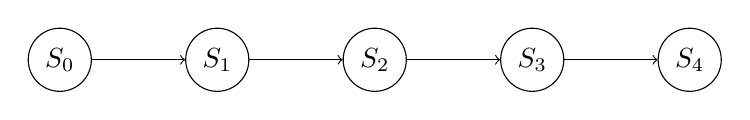
\begin{tikzpicture}
	
	\node[shape=circle,draw=black] (0) at (0,0) {$ S_0 $};
	\node[shape=circle,draw=black] (1) at (2,0) {$ S_1 $};
	\node[shape=circle,draw=black] (2) at (4,0) {$ S_2 $};
	\node[shape=circle,draw=black] (3) at (6,0) {$ S_3 $};
	\node[shape=circle,draw=black] (4) at (8,0) {$ S_4 $};
	
	
	
	\path [->] (0) edge node[left] {} (1);
	\path [->] (1) edge node[left] {} (2);
	\path [->] (2) edge node[left] {} (3);
	\path [->] (3) edge node[left] {} (4);
	
	
	\end{tikzpicture}
\end{center}
A stationary \textit{Markov} chain is described as follows for all $ t > 0 $:
\begin{itemize}
	\item $ P(S_{t+1}| S_0, \dots , S_t) = P(S_{t+1}| S_t)$ (Markov Assumption)
	\item $ P(S_{t+1}| S_t) = P(S_{t'+1}| S_{t'}), \forall t, t' $ (stationary assumption)
\end{itemize}
Consequently, all that needs to be specified is $ P(S_0) $ and $ P(S_{t+1}| S_t) $:
\begin{itemize}
	\item It is a simple Model, easy to specify
	\item It is often the natural model
	\item The network can extend indefinitely
	\item Variations of SMC are at the core of many Natural Language Processing (NLP) applications!
\end{itemize}
\end{document}